% Provenance (never printed): cycle 4 SVT, "La planete Terre, l'environnement
% et l'action humaine": resources from the Earth, their geological origin, the
% time they take to form and the rate we use them; see
% sources/book1/PROVENANCE.md. Book 1, grade 9, chapter 3.
% Vocabulary guard: owns ore deposit (with concentration factor), aggregate,
% reserve. Resource, renewable resource, ore, raw material (chemistry grade
% 5), fossil fuels (chemistry grade 8) and element abundances (chemistry
% grade 9) are recalled in prose. Groundwater and aquifers are g6's. Coal,
% oil and gas are told, not defined: "source rock", "reservoir", "seal",
% "trap" and the coal ranks belong to Book 2 g11 (fossil-fuel-geology);
% "hydrothermal" is not used (later books). Scientific notation (grade 9).
\chapter{Sumber Daya dari Bumi}\label{ch:g9:earth-resources}

Ponsel pintar muat di dalam saku, tetapi di dalamnya terdapat puluhan
unsur kimia: tembaga untuk kabel-kabelnya, neodimium untuk magnet
pengeras suaranya, galium untuk cahaya layarnya, indium untuk lapisan
tipis layarnya yang menghantarkan listrik, dan masih banyak lagi. Setiap
unsur itu digali dari dalam tanah di suatu tempat di Bumi. Sebuah rumah
mengandung jauh lebih banyak lagi: rumah keluarga rata-rata memerlukan
sekitar seratus ton \omterm{def:g3:stones-pebbles-sand:sand}{pasir}, \omterm{def:g3:stones-pebbles-sand:pebble}{kerikil}, dan batu pecah, dan bagiannya dari
jalan dan sekolah di sekitarnya kira-kira tiga kali lipat jumlah itu. Di
bagian Bumi mana bahan-bahan ini ditemukan, dan mengapa di sana?
% ledger: usgs:smartphone, usgs:aggregate (114 and 328 short tons: about 100 and 300 t)

\begin{recall}
Dalam kimia, kamu belajar bahwa bahan-bahan yang kita ambil dari alam
adalah \emph{sumber daya}; \emph{bijih} adalah \omterm{def:g3:stones-pebbles-sand:rock}{batuan} yang darinya logam
dapat diekstraksi; sumber daya yang \emph{terbarukan} diperbarui oleh alam
secepat kita memakainya; batu bara, minyak bumi, dan gas alam adalah
\emph{bahan bakar \omterm{def:g7:sediments-and-fossils:fossil}{fosil}}; dan oksigen, silikon, aluminium, serta besi
adalah unsur-unsur yang paling melimpah di \omterm{def:g6:inside-the-earth:layers}{kerak} bumi. \omterm{def:g6:water-underground:groundwater}{Air tanah} mengisi
\omterm{def:g6:water-underground:porosity}{pori-pori} \omterm{def:g6:water-underground:aquifer}{akuifer}, dan \omterm{def:g4:clouds-rain-snow:precipitation}{hujan} mengisinya kembali
(\cref{ch:g6:water-underground}). \omterm{def:g7:sediments-and-fossils:sediment}{Sedimen} menumpuk berlapis-lapis dan
menjadi \omterm{def:g6:rocks-and-minerals:rock-families}{batuan sedimen} (\cref{ch:g7:sediments-and-fossils}), selama waktu
yang dihitung dalam jutaan tahun (\cref{ch:g7:geological-time}).
\end{recall}

\section{Mengapa logam harus terkonsentrasi}

Tembaga ada di mana-mana: \omterm{def:g3:stones-pebbles-sand:rock}{batuan} biasa mengandung sedikit tembaga,
beberapa gram dalam setiap seratus kilogram. Namun, untuk mendapatkan satu
kilogram tembaga dari \omterm{def:g3:stones-pebbles-sand:rock}{batuan} semacam itu, kamu harus menggali, menghancurkan,
dan mengolah berton-ton \omterm{def:g3:stones-pebbles-sand:rock}{batuan}. Penambangan hanya sepadan dengan biayanya
di tempat alam telah mengumpulkan logam itu ke dalam \omterm{def:g3:stones-pebbles-sand:rock}{batuan} yang jauh
lebih kaya.
% ledger: perkins:ore-grades (copper 0.006 % of the crust)

\begin{definition}[Endapan bijih dan faktor konsentrasi]\label{def:g9:earth-resources:ore-deposit}
Yang disebut \emph{endapan bijih}\index{endapan bijih} adalah tubuh \omterm{def:g3:stones-pebbles-sand:rock}{batuan}
yang di dalamnya proses-proses alam telah mengonsentrasikan suatu logam
atau \omterm{def:g6:rocks-and-minerals:mineral}{mineral} cukup banyak sehingga dapat diekstraksi dengan menguntungkan.
Yang disebut \emph{faktor konsentrasi}\index{faktor konsentrasi} suatu
logam adalah berapa kali kadarnya di dalam bijih lebih besar daripada
kadar rata-ratanya di \omterm{def:g6:inside-the-earth:layers}{kerak} bumi:
\[
\text{faktor konsentrasi} = \frac{\text{kadar di dalam bijih}}{\text{kadar rata-rata di kerak bumi}} .
\]
\end{definition}
% ledger: perkins:ore-grades, earle:ore-grades

Logam-logam yang umum di \omterm{def:g6:inside-the-earth:layers}{kerak} bumi, aluminium dan besi, hanya perlu
dikonsentrasikan sekitar empat kali. Tembaga perlu sekitar 80 kali, seng
sekitar 600 kali, dan logam-logam yang paling langka pada diagram, yaitu
emas, timah, dan kromium, ribuan kali. Makin langka suatu logam di \omterm{def:g6:inside-the-earth:layers}{kerak}
bumi, makin keras alam harus bekerja untuk membentuk bijihnya, dan makin
sedikit tempat yang berhasil dibentuknya.
% ledger: perkins:ore-grades, earle:ore-grades

\begin{example}[Tembaga]
\omterm{def:g6:inside-the-earth:layers}{Kerak} bumi rata-rata mengandung \qty{0.006}{\%} tembaga; bijih tembaga
dapat ditambang mulai dari sekitar \qty{0.5}{\%}. \omterm{def:g9:earth-resources:ore-deposit}{Faktor konsentrasinya}
adalah $0.5 \div 0.006
\approx 83$, sekitar 80, atau mendekati $10^2$. Buku pelajaran lain memakai
\qty{40}{ppm} (\qty{0.004}{\%}) untuk \omterm{def:g3:stones-pebbles-sand:rock}{batuan} biasa dan \qty{1}{\%} untuk
bijihnya: $1 \div
0.004 = 250$. Kedua angka itu berbeda, tetapi keduanya menyatakan hal yang
sama: bijih tembaga kira-kira seratus kali lebih kaya daripada \omterm{def:g3:stones-pebbles-sand:rock}{batuan}
biasa.
\end{example}
% ledger: perkins:ore-grades, earle:ore-grades

\begin{omfigure}
\begin{tikzpicture}
\begin{axis}[xbar, xmode=log, width=12cm, height=5.3cm, xmin=1, xmax=2e4,
  log origin=infty, bar width=9pt, enlarge y limits=0.1,
  ytick=data, yticklabels={aluminium, besi, tembaga, seng, emas, timah, kromium},
  y dir=reverse, xlabel={faktor konsentrasi (skala logaritmik)},
  xtick={1,10,100,1000,10000}, xticklabels={$1$,$10$,$10^2$,$10^3$,$10^4$},
  tick label style={font=\footnotesize}, label style={font=\small},
  nodes near coords, nodes near coords style={font=\scriptsize, anchor=west},
  point meta=explicit, xmajorgrids, grid style={black!12}]
\addplot[fill=omWarm!45, draw=omWarm!80!black] table[x=factor, y=x, meta=factor] {figdata/out/grade-9-concentration.dat};
\end{axis}
\end{tikzpicture}

{\small Berapa kali alam harus mengonsentrasikan tujuh logam untuk
membentuk bijih yang layak ditambang: kadar minimum bijih dibagi dengan
kadar rata-rata \omterm{def:g6:inside-the-earth:layers}{kerak} bumi. Setiap langkah skala sepuluh kali langkah
sebelumnya. Data: D.~Perkins dan kawan-kawan, \emph{Mineralogy}, dan,
untuk emas, S.~Earle, \emph{Environmental Geology}.}
% ledger: perkins:ore-grades, earle:ore-grades (figdata/grade-9/concentration.py)
\label{fig:g9:earth-resources:factors}
\end{omfigure}

\begin{method}[Menghitung faktor konsentrasi]
\begin{enumerate}
  \item Tuliskan kadar logam di dalam bijih dan di dalam \omterm{def:g6:inside-the-earth:layers}{kerak} bumi
        rata-rata dalam satuan yang sama (persen, atau gram per ton).
  \item Bagilah kadar di dalam bijih dengan kadar di dalam \omterm{def:g6:inside-the-earth:layers}{kerak} bumi.
  \item Bulatkan hasilnya: yang penting adalah besarnya, sekitar 10, 100,
        atau 1000, yang dapat kamu tuliskan sebagai pangkat sepuluh.
\end{enumerate}
\end{method}


\section{Bagaimana endapan bijih terbentuk}

Alam mengonsentrasikan logam dengan beberapa cara. Tiga di antaranya ditunjukkan di bawah ini.

\begin{omfigure}
\begin{tikzpicture}[x=1cm, y=1cm, font=\footnotesize, >={Stealth[length=2mm]}]
  % country rock
  \fill[black!13] (0,0) rectangle (13,4.6);
  % surface with a valley on the right
  \fill[white] (0,4.6) -- (8.4,4.6) -- (9.6,3.7) -- (11.2,3.7) -- (12.0,4.6) -- (13,4.6) -- (13,5.6) -- (0,5.6) -- cycle;
  \draw[black!60] (0,4.6) -- (8.4,4.6) -- (9.6,3.7) -- (11.2,3.7) -- (12.0,4.6) -- (13,4.6);
  % river gravels on the valley floor
  \fill[omLithCongl] (9.5,3.75) -- (11.3,3.75) -- (11.15,3.35) -- (9.65,3.35) -- cycle;
  \foreach \x in {9.8,10.1,10.45,10.8,11.05} \fill[black!45] (\x,3.6) circle (0.05);
  \foreach \x in {9.9,10.3,10.65,10.95} \fill[yellow!80!orange] (\x,3.4) circle (0.045);
  \fill[omRiver!60] (9.9,3.75) rectangle (10.9,3.85);
  % magma body (cooling granite)
  \fill[omLithGranite] (1.0,0) .. controls (1.2,1.6) and (2.2,2.1) .. (3.4,2.1)
     .. controls (4.6,2.1) and (5.6,1.6) .. (5.8,0) -- cycle;
  \draw[black!50] (1.0,0) .. controls (1.2,1.6) and (2.2,2.1) .. (3.4,2.1)
     .. controls (4.6,2.1) and (5.6,1.6) .. (5.8,0);
  % heavy minerals settled at the bottom of the magma body
  \fill[black!60] (1.05,0) rectangle (5.75,0.25);
  % cracks and veins above the magma
  \foreach \x/\a in {2.6/12, 3.4/-6, 4.3/-15} {
    \draw[black, line width=1.6pt] (\x,2.15) -- ++(90+\a:2.0);
    \draw[yellow!80!orange, line width=0.6pt] (\x,2.15) -- ++(90+\a:2.0);
  }
  % hot water rising
  \draw[->, omWarm, thick] (2.1,1.9) .. controls (1.9,2.7) and (2.2,3.2) .. (2.45,3.7);
  \draw[->, omWarm, thick] (4.95,1.7) .. controls (5.1,2.6) and (4.8,3.3) .. (4.55,3.8);
  % labels
  \node[anchor=north, align=center] at (3.4,1.35) {tubuh magma\\ yang mendingin};
  \node[anchor=west, align=left, fill=white, fill opacity=0.85, text opacity=1, inner sep=1.5pt] at (6.2,0.75)
    {\textbf{1} mineral berat yang kaya logam\\ mengendap di dasar};
  \draw[black!70] (6.15,0.65) -- (5.5,0.15);
  \node[anchor=west, align=left, fill=white, fill opacity=0.85, text opacity=1, inner sep=1.5pt] at (5.6,2.55)
    {\textbf{2} air panas naik melalui retakan,\\ mendingin, dan meninggalkan logam: urat};
  \draw[black!70] (5.55,2.6) -- (4.2,3.3);
  \node[anchor=south, align=center] at (10.4,4.7) {\textbf{3} butir-butir emas mengendap bersama\\ kerikil sungai: endapan plaser};
  \draw[black!70] (10.4,4.7) -- (10.3,3.45);
  \node[anchor=south west] at (0.1,4.65) {permukaan tanah};
\end{tikzpicture}

{\small Tiga cara mengonsentrasikan logam (sketsa, tidak berskala). (1) Di
dalam tubuh \omterm{def:g7:volcanoes:magma}{magma}, \omterm{def:g6:rocks-and-minerals:mineral}{mineral} berat yang kaya nikel atau tembaga tenggelam
dan berkumpul di dasar. (2) \omterm{def:g6:water-underground:groundwater}{Air tanah} yang dipanaskan oleh \omterm{def:g7:volcanoes:magma}{magma}, dan air
yang dilepaskan oleh \omterm{def:g7:volcanoes:magma}{magma} itu sendiri, melarutkan logam, naik melalui
retakan, lalu menjatuhkan logam itu di tempat \omterm{def:g3:stones-pebbles-sand:rock}{batuannya} lebih dingin,
sehingga retakan-retakan itu terisi urat. (3) \omterm{def:g5:water-shapes-the-land:erosion}{Erosi} membebaskan emas dari
urat; \omterm{def:g1:landscapes-around-us:water}{sungai} membawanya, dan butir-butir yang berat mengendap di antara
\omterm{def:g3:stones-pebbles-sand:pebble}{kerikil}, sampai ke \omterm{def:g3:stones-pebbles-sand:rock}{batuan dasar}.}
% ledger: earle:magmatic, usgs:gold-lode, usgs:gold-placer
\label{fig:g9:earth-resources:deposits}
\end{omfigure}

\paragraph{Di dalam magma.} Ketika tubuh \omterm{def:g7:volcanoes:magma}{magma} mendingin, \omterm{def:g6:rocks-and-minerals:mineral}{mineral} yang
pertama kali mengkristal tidak selalu yang paling ringan. Di dalam \omterm{def:g7:volcanoes:magma}{magma}
yang berasal dari \omterm{def:g6:inside-the-earth:layers}{mantel}, \omterm{def:g6:rocks-and-minerals:mineral}{mineral} berat yang kaya nikel dan tembaga
tenggelam ke dasar dan berkumpul membentuk lapisan yang kaya. Sebagian
besar nikel yang ditambang di dunia berasal dari endapan jenis ini.
% ledger: earle:magmatic

\paragraph{Di dalam retakan, dari air panas.} \omterm{def:g6:water-underground:groundwater}{Air tanah} yang mengalir di
dekat tubuh \omterm{def:g7:volcanoes:magma}{magma}, beberapa kilometer di bawah permukaan, menjadi panas
dan naik melalui retakan-retakan \omterm{def:g3:stones-pebbles-sand:rock}{batuan}. Air panas melarutkan logam dari
\omterm{def:g3:stones-pebbles-sand:rock}{batuan} yang dilaluinya. Ketika air itu mencapai \omterm{def:g3:stones-pebbles-sand:rock}{batuan} yang lebih dingin
di dekat permukaan, logam-logam itu keluar dari air sebagai \omterm{def:g6:rocks-and-minerals:mineral}{mineral} dan
mengisi retakan: inilah \emph{urat}\index{urat (bijih)}. Banyak endapan
emas berupa urat jenis ini. Di sekitar beberapa tubuh \omterm{def:g7:volcanoes:magma}{magma}, air panas
telah melintasi seluruh massa \omterm{def:g3:stones-pebbles-sand:rock}{batuan} yang retak-retak dan meninggalkan
tembaga di dalamnya, tersebar tetapi dalam volume yang sangat besar:
inilah endapan tembaga terbesar di dunia.
% ledger: usgs:gold-lode, earle:porphyry

\begin{omfigure}
\begin{minipage}[c]{0.46\linewidth}\centering
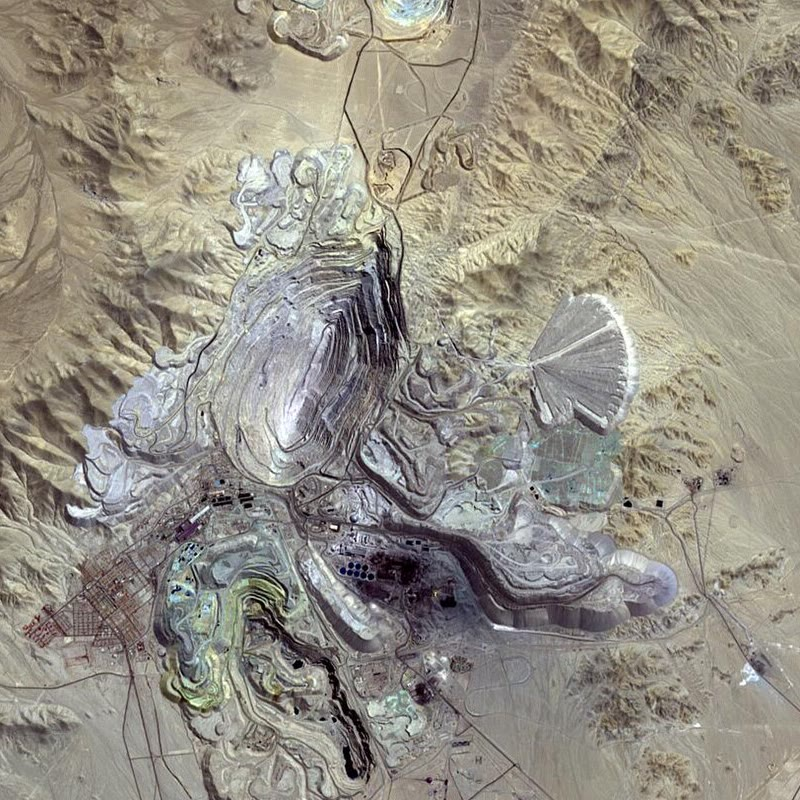
\includegraphics[width=\linewidth]{images/book1/g9-chuquicamata.jpg}
\end{minipage}\hfill
\begin{minipage}[c]{0.5\linewidth}\raggedright
{\small Tambang tembaga Chuquicamata, di \omterm{def:g5:weather-and-climate:desert}{Gurun} Atacama, Chili, yang
dipotret oleh instrumen ASTER pada sebuah satelit NASA pada tahun 2007
(lebar citra itu sekitar \qty{12}{km}). Lubang tambang lonjong di
tengahnya, yang telah ditambang selama lebih dari seabad, panjangnya
\qty{4.3}{km}, lebarnya \qty{2.7}{km}, dan dalamnya \qty{1.1}{km}.
NASA/METI/AIST/Japan Space Systems dan U.S./Japan ASTER Science Team
(domain publik, melalui Wikimedia Commons).}
\end{minipage}
% ledger: commons:chuquicamata, earle:chuquicamata
\label{fig:g9:earth-resources:chuquicamata}
\end{omfigure}

\paragraph{Di dalam kerikil sungai.} Emas tidak berkarat dan hampir tidak
melapuk. Ketika \omterm{def:g5:water-shapes-the-land:erosion}{erosi} mengikis urat emas, emasnya terbebaskan sebagai
debu, serpihan, butiran, dan kadang-kadang bongkahan, lalu \omterm{def:g1:landscapes-around-us:water}{sungai}
membawanya ke hilir. Emas sangat rapat: sekitar \qty{19}{g/cm^3} jika
murni, dibandingkan dengan sekitar \qty{2.5}{g/cm^3} untuk \omterm{def:g3:stones-pebbles-sand:rock}{batuan} biasa.
Pada saat \omterm{def:g5:water-shapes-the-land:flood}{banjir}, ketika seluruh dasar \omterm{def:g3:stones-pebbles-sand:sand}{pasir} dan \omterm{def:g3:stones-pebbles-sand:pebble}{kerikil} bergerak,
butir-butir emas yang berat perlahan-lahan turun dan berkumpul di atas
\omterm{def:g3:stones-pebbles-sand:rock}{batuan dasar}. Para ahli geologi menyebut endapan semacam itu
\emph{endapan plaser}\index{endapan plaser}.
% ledger: usgs:gold-placer

\section{Batu bara, minyak bumi, dan gas alam}

Batu bara, minyak bumi, dan gas alam adalah sisa-sisa makhluk hidup yang
terkubur sebelum sempat membusuk. Hampir semua bahan organik tumbuhan atau
hewan yang mati kembali menjadi karbon dioksida dalam waktu beberapa
minggu sampai beberapa dasawarsa. Hanya bagian yang terputus dari oksigen
udara, di dasar rawa yang airnya tergenang atau di dasar \omterm{def:g2:water-on-earth:ocean}{laut} dalam, yang
dapat terkubur dan tersimpan selama jutaan tahun.
% ledger: earle:coal, earle:oil-gas

\begin{omfigure}
\begin{minipage}[c]{0.46\linewidth}\centering
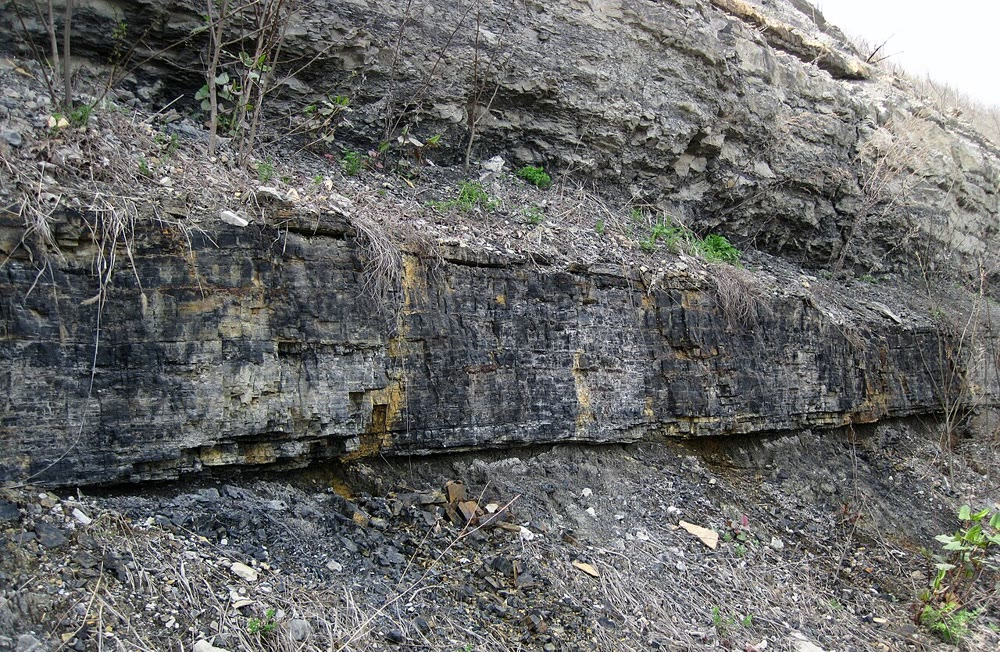
\includegraphics[width=\linewidth]{images/book1/g9-coal-seam.jpg}
\end{minipage}\hfill
\begin{minipage}[c]{0.5\linewidth}\raggedright
{\small Lapisan batu bara, yaitu lapisan gelap yang melintang di tengah,
di antara \omterm{def:g6:rocks-and-minerals:rock-families}{batuan sedimen}, di tepi sebuah jalan di Ohio, Amerika Serikat.
Lapisan itu mendatar, sebagaimana rawanya dahulu. Foto oleh James St.~John
(CC BY 2.0, melalui Wikimedia Commons).}
\end{minipage}
% ledger: commons:meigs-coal
\label{fig:g9:earth-resources:coal-seam}
\end{omfigure}


\paragraph{Batu bara.} Batu bara bermula di rawa-rawa di tepi \omterm{def:g1:landscapes-around-us:water}{sungai} dan
\omterm{def:g5:water-shapes-the-land:delta}{delta}, pada \omterm{def:g5:weather-and-climate:climate}{iklim} yang hangat dan basah, tempat tumbuhan tumbuh dengan
cepat. Batang dan daun yang mati jatuh ke dalam air tenang yang sedikit
oksigennya, dan tidak membusuk. Rawa itu harus bertahan selama berabad-abad
sampai beribu-ribu tahun untuk membentuk lapisan yang tebal. Suatu hari,
\omterm{def:g1:landscapes-around-us:water}{sungai} berpindah alur atau \omterm{def:g5:water-shapes-the-land:flood}{banjir}, lalu menutupi rawa itu dengan \omterm{def:g3:stones-pebbles-sand:sand}{pasir} dan
\omterm{def:g3:stones-pebbles-sand:sand}{lumpur}. Selagi makin banyak \omterm{def:g7:sediments-and-fossils:sediment}{sedimen} menumpuk, lapisan tumbuhan itu
tertekan dan terpanaskan, lalu berubah menjadi batu bara: mula-mula batu
bara cokelat yang lunak dengan kadar karbon sekitar sepertiga, beberapa
ratus meter di bawah permukaan; lalu batu bara hitam yang keras, dengan
kadar karbon sampai 86~\%, beberapa kilometer di bawah permukaan. Batu bara
yang ditambang sekarang di Amerika Serikat, misalnya, sebagian besar
berumur 100 sampai 300~juta tahun.
% ledger: earle:coal, eia:coal

\begin{omfigure}
\begin{tikzpicture}[x=1cm, y=0.8cm, font=\footnotesize]
  \foreach \i/\t in {0/{(a) hutan rawa:\\ tumbuhan mati\\ menumpuk di bawah\\ air tenang},
                     1/{(b) terkubur di\\ bawah pasir dan\\ lumpur sungai:\\ lapisan tertekan},
                     2/{(c) lebih dalam,\\ lebih panas\\ (ratusan meter):\\ batu bara cokelat\\ yang lunak},
                     3/{(d) lebih dalam lagi\\ (berkilo-kilometer):\\ batu bara\\ hitam keras}} {
    \begin{scope}[xshift=\i*3.35cm]
      \draw[black!40] (0,0) rectangle (2.9,4.2);
      \node[align=center, anchor=north, font=\scriptsize] at (1.45,-0.1) {\t};
    \end{scope}
  }
  % (a) swamp: water, trees, plant layer
  \fill[omSea] (0,2.6) rectangle (2.9,3.1);
  \fill[brown!60!black!70] (0,2.0) rectangle (2.9,2.6);
  \fill[omLithShale] (0,0) rectangle (2.9,2.0);
  \foreach \x in {0.5,1.4,2.3} {
    \draw[brown!50!black, line width=1.2pt] (\x,2.6) -- (\x,3.7);
    \fill[green!45!black] (\x,3.85) circle (0.3);
  }
  % (b) buried
  \begin{scope}[xshift=3.35cm]
    \fill[lith sandstone] (0,2.6) rectangle (2.9,4.0);
    \fill[brown!55!black!80] (0,2.2) rectangle (2.9,2.6);
    \fill[omLithShale] (0,0) rectangle (2.9,2.2);
    \draw[->, thick] (1.45,4.15) -- (1.45,3.45);
  \end{scope}
  % (c) lignite
  \begin{scope}[xshift=6.7cm]
    \fill[lith sandstone] (0,1.9) rectangle (2.9,4.2);
    \fill[brown!45!black] (0,1.65) rectangle (2.9,1.9);
    \fill[omLithShale] (0,0) rectangle (2.9,1.65);
  \end{scope}
  % (d) coal
  \begin{scope}[xshift=10.05cm]
    \fill[lith sandstone] (0,1.25) rectangle (2.9,4.2);
    \fill[black!85] (0,1.1) rectangle (2.9,1.25);
    \fill[omLithShale] (0,0) rectangle (2.9,1.1);
  \end{scope}
\end{tikzpicture}

{\small Dari rawa menjadi lapisan batu bara (sketsa, tidak berskala).
Selagi lapisan tumbuhan tenggelam makin dalam, lapisan itu tertekan dan
terpanaskan: air dan gas keluar darinya, lapisan itu menipis, dan kadar
karbonnya naik.}
% ledger: earle:coal, eia:coal
\label{fig:g9:earth-resources:coal}
\end{omfigure}


\paragraph{Minyak bumi dan gas alam.} Minyak bumi dan sebagian besar gas
alam berasal dari tumbuhan dan hewan renik yang hidup di \omterm{def:g2:water-on-earth:ocean}{laut}, seperti
diatom. Sisa-sisanya tenggelam bersama \omterm{def:g3:stones-pebbles-sand:sand}{lumpur} ke dasar \omterm{def:g2:water-on-earth:ocean}{laut}, dan sebagian
terkubur sebelum membusuk. Jutaan tahun dan berkilo-kilometer \omterm{def:g7:sediments-and-fossils:sediment}{sedimen}
kemudian, panas dan tekanan mengubahnya: di bawah kedalaman sekitar
\qty{2}{km}, pada suhu antara sekitar 60 dan \qty{120}{\degreeCelsius},
menjadi minyak bumi; pada suhu yang lebih panas lagi, menjadi gas. Minyak
bumi dan gas alam lebih ringan daripada air. Keduanya merayap perlahan ke
atas melalui \omterm{def:g6:water-underground:porosity}{pori-pori} \omterm{def:g3:stones-pebbles-sand:rock}{batuan} yang \omterm{def:g6:water-underground:permeability}{permeabel}, dan banyak yang mencapai
permukaan lalu hilang. Yang kita temukan adalah yang tertahan di
perjalanannya oleh lapisan \omterm{def:g3:stones-pebbles-sand:rock}{batuan} yang kedap, sering kali di puncak
lipatan yang melengkung ke atas, tempat keduanya berkumpul: gas di bagian
atas, minyak di bawahnya, dan air di bawah minyak.
% ledger: eia:oil, eia:gas, earle:oil-gas

\begin{omfigure}
\begin{tikzpicture}[x=1cm, y=1cm, font=\footnotesize, >={Stealth[length=2mm]}]
  \def\fold#1{(0,#1) .. controls (3,#1+1.0) and (4.0,#1+1.6) .. (6,#1+1.6) .. controls (8.0,#1+1.6) and (9,#1+1.0) .. (12,#1)}
  % layers from the bottom up
  \fill[omLithShale!60!black!40] (0,0) -- \fold{0.9} -- (12,0) -- cycle;
  \fill[lith sandstone] \fold{0.9} -- (12,2.1) -- (12,2.1) .. controls (9,3.1) and (8.0,3.7) .. (6,3.7) .. controls (4.0,3.7) and (3,3.1) .. (0,2.1) -- cycle;
  \fill[lith shale] (0,2.1) .. controls (3,3.1) and (4.0,3.7) .. (6,3.7) .. controls (8.0,3.7) and (9,3.1) .. (12,2.1) -- (12,3.6) .. controls (9,4.6) and (8.0,5.2) .. (6,5.2) .. controls (4.0,5.2) and (3,4.6) .. (0,3.6) -- cycle;
  \fill[lith sandstone] (0,3.6) .. controls (3,4.6) and (4.0,5.2) .. (6,5.2) .. controls (8.0,5.2) and (9,4.6) .. (12,3.6) -- (12,5.6) -- (0,5.6) -- cycle;
  % gas and oil under the crest of the impermeable layer
  \fill[omWxSun!60] (4.55,3.55) .. controls (5.2,3.69) and (6.8,3.69) .. (7.45,3.55) -- (7.1,3.35) -- (4.9,3.35) -- cycle;
  \fill[black!75] (4.9,3.35) -- (7.1,3.35) -- (8.05,3.05) .. controls (7.0,3.15) and (5.0,3.15) .. (3.95,3.05) -- cycle;
  % arrows: oil creeping up through the permeable layer
  \draw[->, black, thick] (1.4,2.05) -- (2.4,2.55);
  \draw[->, black, thick] (10.6,2.05) -- (9.6,2.55);
  \draw[->, black!70] (3.0,2.65) -- (3.8,2.95);
  \draw[->, black!70] (9.0,2.65) -- (8.2,2.95);
  % labels
  \node[anchor=west, fill=white, fill opacity=0.85, text opacity=1, inner sep=1.5pt] at (0.1,0.45) {lumpur gelap dasar laut purba: minyak dan gas terbentuk di sini};
  \node[anchor=east, fill=white, fill opacity=0.85, text opacity=1, inner sep=1.5pt] at (11.9,1.9) {batu pasir yang permeabel};
  \node[anchor=east, fill=white, fill opacity=0.85, text opacity=1, inner sep=1.5pt] at (11.9,3.25) {serpih yang kedap};
  \node[anchor=south, fill=white, fill opacity=0.85, text opacity=1, inner sep=1.5pt] at (6,5.25) {batuan permukaan};
  \node[font=\scriptsize] at (6,3.48) {gas};
  \node[font=\scriptsize, text=white] at (6,3.22) {minyak};
\end{tikzpicture}

{\small Minyak bumi dan gas alam yang tertahan di bawah lapisan yang kedap
di puncak lipatan yang melengkung ke atas (sketsa, tidak berskala; air
yang mengisi bagian batu pasir lainnya tidak digambar). Di bawah lipatan,
keduanya merayap naik melalui batu pasir yang \omterm{def:g6:water-underground:permeability}{permeabel} (panah) dan
berkumpul di bawah puncaknya: gas di atas, minyak di bawahnya.}
% ledger: earle:oil-gas
\label{fig:g9:earth-resources:oil}
\end{omfigure}

\section{Air dari dalam tanah}

\omterm{def:g6:water-underground:groundwater}{Air tanah} juga merupakan sumber daya dari Bumi, yang kita pakai setiap
hari. Tidak seperti logam atau batu bara, \omterm{def:g6:water-underground:groundwater}{air tanah} diperbarui: \omterm{def:g4:clouds-rain-snow:precipitation}{hujan}
mengisi kembali \omterm{def:g6:water-underground:aquifer}{akuifer}. Namun, pembaruannya lambat, dan hanya secepat
\omterm{def:g4:clouds-rain-snow:precipitation}{hujan} meresap. \omterm{def:g6:water-underground:aquifer}{Akuifer} yang dipompa lebih cepat daripada pengisiannya
kembali mengalami penurunan \omterm{def:g6:water-underground:water-table}{muka air tanah}, dan \omterm{def:g6:water-underground:spring}{sumur-sumur} menjadi kering
(\cref{ch:g6:water-underground}). \omterm{def:g6:water-underground:groundwater}{Air tanah} adalah sumber daya terbarukan
hanya selama air itu tidak diambil lebih cepat daripada pembaruannya.
% ledger: wss:aquifer

\section{Pasir dan kerikil}

Bahan padat yang paling banyak digali manusia dari dalam tanah bukanlah
batu bara ataupun bijih logam, melainkan \omterm{def:g3:stones-pebbles-sand:sand}{pasir} dan \omterm{def:g3:stones-pebbles-sand:pebble}{kerikil}.
% ledger: tos:sand

\begin{definition}[Agregat]\label{def:g9:earth-resources:aggregate}
Yang disebut \emph{agregat}\index{agregat} adalah \omterm{def:g3:stones-pebbles-sand:sand}{pasir}, \omterm{def:g3:stones-pebbles-sand:pebble}{kerikil}, dan
batu pecah yang dipakai dalam pembangunan: di dalam beton, di bawah jalan
raya dan rel kereta api, dan untuk menimbun tanah.
\end{definition}
% ledger: usgs:aggregate, tos:sand

Sebagian besar \omterm{def:g3:stones-pebbles-sand:sand}{pasir} dipakai untuk beton, campuran \omterm{def:g3:stones-pebbles-sand:sand}{pasir}, \omterm{def:g3:stones-pebbles-sand:pebble}{kerikil}, air,
dan semen. Pada tahun 2019, dunia memerlukan sekitar 50~miliar ton \omterm{def:g3:stones-pebbles-sand:sand}{pasir}
dan \omterm{def:g3:stones-pebbles-sand:pebble}{kerikil} setahun, yaitu $5 \times 10^{10}$ ton, atau sekitar
\qty{18}{kg} untuk setiap orang di Bumi, setiap hari. \omterm{def:g3:stones-pebbles-sand:sand}{Pasir} dan \omterm{def:g3:stones-pebbles-sand:pebble}{kerikil}
digali dari lubang galian di darat, dari dasar \omterm{def:g1:landscapes-around-us:water}{sungai}, dan, makin lama
makin banyak, dari dasar \omterm{def:g2:water-on-earth:ocean}{laut}. Jika diambil dari \omterm{def:g1:landscapes-around-us:water}{sungai}, makin sedikit
\omterm{def:g3:stones-pebbles-sand:sand}{pasir} yang sampai ke pantai, dan pantai-pantai di hilir terkikis.
% ledger: tos:sand

\begin{omfigure}
\begin{minipage}[c]{0.46\linewidth}\centering
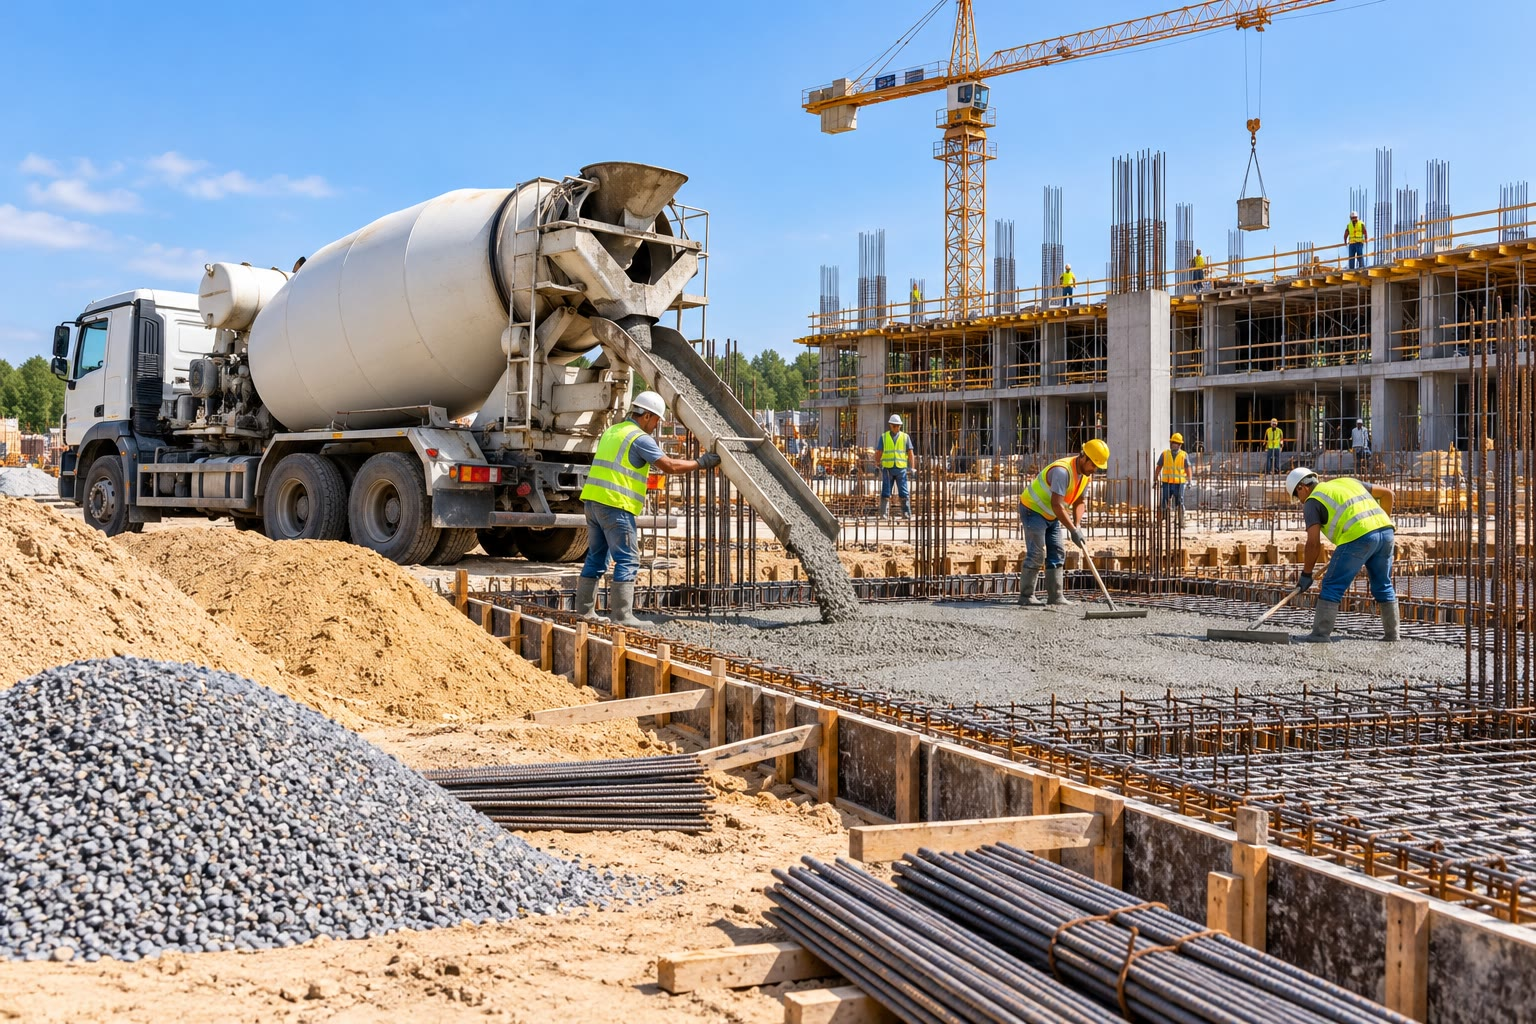
\includegraphics[width=\linewidth]{images/book1/ai/g9-building-site.jpg}
\end{minipage}\hfill
\begin{minipage}[c]{0.5\linewidth}\raggedright
{\small \omterm{def:g9:earth-resources:aggregate}{Agregat} yang sedang dipakai: timbunan \omterm{def:g3:stones-pebbles-sand:sand}{pasir} dan \omterm{def:g3:stones-pebbles-sand:pebble}{kerikil} di samping
truk molen yang sedang menuangkan beton untuk lantai sebuah bangunan baru
(ilustrasi AI dari suatu adegan umum).}
\end{minipage}
\label{fig:g9:earth-resources:building-site}
\end{omfigure}

\section{Terbarukan atau terbatas?}

Sumber daya yang diperbarui alam dalam rentang hidup manusia, seperti air
\omterm{def:g6:water-underground:aquifer}{akuifer} yang tidak dipompa berlebihan, dapat dipakai selamanya. \omterm{def:g9:earth-resources:ore-deposit}{Endapan
bijih}, lapisan batu bara, atau ladang minyak memerlukan jutaan tahun untuk
terbentuk. Kita memakainya dalam beberapa dasawarsa: pada skala waktu
kita, sumber daya itu sama sekali tidak diperbarui.
% ledger: eia:coal, earle:coal

\begin{omfigure}
\begin{tikzpicture}
\begin{axis}[xmode=log, width=12.5cm, height=4.6cm, xmin=10, xmax=1e9, ymin=0.4, ymax=4.6,
  ytick=\empty, xlabel={tahun (skala logaritmik)}, label style={font=\small},
  xtick={10,100,1000,1e4,1e5,1e6,1e7,1e8,1e9},
  xticklabels={$10$,$10^2$,$10^3$,$10^4$,$10^5$,$10^6$,$10^7$,$10^8$,$10^9$},
  tick label style={font=\footnotesize}, xmajorgrids, grid style={black!12}, clip=false]
\addplot[only marks, mark=|, mark size=4pt, line width=4pt, omWarm,
  error bars/.cd, x dir=plus, x explicit, error bar style={line width=4pt, omWarm}, error mark=none]
  table[x=lo_yr, y=y, x error expr=\thisrow{hi_yr}-\thisrow{lo_yr}] {figdata/out/grade-9-concentration-times.dat};
\node[anchor=west, font=\footnotesize, fill=white, inner sep=1pt] at (axis cs:1500,4) {rawa membentuk lapisan tumbuhan yang tebal};
\node[anchor=east, font=\footnotesize, fill=white, inner sep=1pt] at (axis cs:6e7,3) {umur batu bara yang ditambang di Amerika Serikat};
\node[anchor=west, font=\footnotesize, fill=white, inner sep=1pt] at (axis cs:150,2) {Chuquicamata, ditambang sampai sekarang (lebih dari seabad)};
\node[anchor=west, font=\footnotesize, fill=white, inner sep=1pt] at (axis cs:65,1) {cadangan tembaga dunia dengan laju penambangan 2024};
\end{axis}
\end{tikzpicture}

{\small Waktu pembentukan dan waktu pemakaian, pada skala yang setiap
langkahnya sepuluh kali langkah sebelumnya. Batu bara itu kira-kira sejuta
kali lebih tua daripada waktu yang diperlukan sebuah tambang untuk
mengosongkan suatu endapan.}
% ledger: earle:coal, eia:coal, earle:chuquicamata, usgs:mcs-copper (figdata/grade-9/concentration.py, part times)
\label{fig:g9:earth-resources:times}
\end{omfigure}

Berapa lama suatu sumber daya akan bertahan? Para ahli geologi hanya
menghitung apa yang sudah diketahui dan dapat diekstraksi.

\begin{definition}[Cadangan]\label{def:g9:earth-resources:reserve}
Yang disebut \emph{cadangan}\index{cadangan} suatu sumber daya \omterm{def:g6:rocks-and-minerals:mineral}{mineral}
adalah bagian dari endapan-endapan yang sudah diketahui yang dapat
diekstraksi dengan menguntungkan, dengan teknik dan harga pada masa itu.
\end{definition}
% ledger: usgs:mcs-reserves

\omterm{def:g9:earth-resources:reserve}{Cadangan} bukanlah segala sesuatu yang ada di dalam tanah. \omterm{def:g9:earth-resources:reserve}{Cadangan}
bertambah ketika endapan baru ditemukan, ketika teknik membaik, atau
ketika harga naik, dan berkurang selagi endapan-endapan ditambang. Pada
tahun 1970, \omterm{def:g9:earth-resources:reserve}{cadangan} tembaga dunia diperkirakan sebesar 280~juta ton.
Sejak itu, sekitar 700~juta ton tembaga telah ditambang, dua setengah kali
\omterm{def:g9:earth-resources:reserve}{cadangan} itu, tetapi \omterm{def:g9:earth-resources:reserve}{cadangan} tahun 2024 diperkirakan sebesar 980~juta
ton.
% ledger: usgs:mcs-reserves

\begin{dated}{2025}
Pada tahun 2024, tambang-tambang di dunia menghasilkan sekitar 23~juta ton
tembaga. Dengan laju itu, \omterm{def:g9:earth-resources:reserve}{cadangan} sebesar 980~juta ton akan bertahan
$980 \div 23
\approx 43$ tahun. Angka seperti itu bukanlah tanggal habisnya tembaga:
angka itu adalah ukuran tembaga yang sudah diketahui dan layak diekstraksi
sekarang.
\end{dated}
% ledger: usgs:mcs-copper (figdata/grade-9/concentration.py: 42.6 years)

Logam, tidak seperti batu bara atau minyak bumi, tidak musnah ketika
dipakai: daur ulang bahan, yang dibahas dalam buku-buku kimia,
mengembalikannya. Tembaga dari kabel bekas, dari mesin rongsokan, atau
dari potongan sisa sebuah pabrik dapat dilebur dan dimurnikan lagi. Di
Amerika Serikat pada tahun 2024, tembaga yang diperoleh kembali dari
barang bekas mencakup sekitar \qty{35}{\%} dari seluruh tembaga yang
dipakai.
% ledger: usgs:mcs-copper-scrap

\begin{omfigure}
\begin{tikzpicture}[font=\footnotesize, node distance=1.2cm,
  box/.style={draw=black!60, fill=black!4, rounded corners=2pt, align=center, minimum height=0.9cm, inner sep=3pt},
  flow/.style={-{Stealth[length=2.2mm]}, line width=0.9pt, black!70}]
  \node[box, fill=omWarm!12] (ore) at (0,0) {endapan bijih\\(batuan dengan \qty{0.5}{\%}\\tembaga)};
  \node[box] (metal) at (4.2,0) {logam tembaga};
  \node[box] (things) at (8.2,0) {kabel, pipa,\\mesin};
  \node[box, fill=blue!8] (scrap) at (6.2,-2.1) {barang bekas};
  \node[box, fill=black!12] (waste) at (0,-2.1) {sisa batuan\\yang dihancurkan};
  \draw[flow] (ore) -- node[above] {gali, hancurkan,} node[below] {konsentrasikan} (metal);
  \draw[flow] (metal) -- node[above] {buat} (things);
  \draw[flow] (things) |- node[pos=0.25, right] {dibuang} (scrap);
  \draw[flow] (scrap) -| node[pos=0.75, left] {lebur, murnikan} (metal);
  \draw[flow] (ore) -- (waste);
\end{tikzpicture}

{\small Dua jalan menuju logam tembaga: dari bijih, melalui berton-ton
\omterm{def:g3:stones-pebbles-sand:rock}{batuan} yang digali dan dihancurkan, atau dari barang bekas, yang dilebur
dan dimurnikan lagi.}
\end{omfigure}

\begin{example}[Batuan yang diselamatkan oleh daur ulang]\label{ex:g9:earth-resources:recycling}
Bijih dengan \qty{0.5}{\%} tembaga mengandung \qty{5}{kg} tembaga dalam
setiap ton \omterm{def:g3:stones-pebbles-sand:rock}{batuan}. Untuk membuat satu ton tembaga, sekitar
$1000 \div 5 = 200$ ton bijih harus digali, dihancurkan, dan diolah, dan
hampir semuanya berakhir sebagai \omterm{def:g3:stones-pebbles-sand:rock}{batuan} buangan. Setiap ton tembaga yang
dibuat dari barang bekas membiarkan 200 ton \omterm{def:g3:stones-pebbles-sand:rock}{batuan} itu tetap di dalam
tanah --- dan endapan itu bertahan lebih lama.
% ledger: perkins:ore-grades (computed)
\end{example}


\section{Latihan}

\begin{exercise}[$\star$]\label{exo:g9:earth-resources:1}
Lengkapilah dengan kata yang tepat (\omterm{def:g9:earth-resources:ore-deposit}{endapan bijih}, \omterm{def:g9:earth-resources:ore-deposit}{faktor konsentrasi},
\omterm{def:g9:earth-resources:aggregate}{agregat}, \omterm{def:g9:earth-resources:reserve}{cadangan}). (a) \omterm{def:g3:stones-pebbles-sand:sand}{Pasir} yang dipakai di dalam beton adalah
\ldots\ (b) Bagian dari tembaga yang sudah diketahui yang dapat
diekstraksi dengan menguntungkan sekarang adalah \ldots\ tembaga. (c) \omterm{def:g3:stones-pebbles-sand:rock}{Batuan}
yang di dalamnya suatu logam cukup kaya untuk ditambang adalah
\ldots\ (d) Bilangan yang menyatakan berapa kali suatu logam telah
dikonsentrasikan adalah \ldots\ logam itu.
\end{exercise}

\begin{exercise}[$\star$]\label{exo:g9:earth-resources:2}
% ledger: earle:magmatic, usgs:gold-lode, usgs:gold-placer
Cara mengonsentrasikan logam yang mana yang digambarkan setiap kalimat:
di dalam \omterm{def:g7:volcanoes:magma}{magma}, di dalam retakan dari air panas, atau di dalam \omterm{def:g3:stones-pebbles-sand:pebble}{kerikil}
\omterm{def:g1:landscapes-around-us:water}{sungai}? (a) Bongkahan emas tergeletak di atas \omterm{def:g3:stones-pebbles-sand:rock}{batuan dasar} di bawah
\omterm{def:g3:stones-pebbles-sand:pebble}{kerikil} sebuah \omterm{def:g1:landscapes-around-us:water}{sungai} kecil. (b) Air panas mengisi sebuah retakan dengan
kuarsa dan emas. (c) Lapisan \omterm{def:g6:rocks-and-minerals:mineral}{mineral} nikel yang berat terletak di dasar
sebuah tubuh \omterm{def:g7:volcanoes:magma}{magma} purba. (d) Emas dibebaskan dari urat oleh \omterm{def:g5:water-shapes-the-land:erosion}{erosi}.
\end{exercise}

\begin{exercise}[$\star$]\label{exo:g9:earth-resources:3}
% ledger: earle:coal, eia:coal
Urutkan langkah-langkah ini: (a) lapisan tumbuhan terkubur di bawah \omterm{def:g3:stones-pebbles-sand:sand}{pasir}
\omterm{def:g1:landscapes-around-us:water}{sungai}; (b) pohon-pohon tumbuh di rawa; (c) batu bara hitam yang keras
terbentuk berkilo-kilometer di bawah permukaan; (d) tumbuhan mati
menumpuk di bawah air tenang; (e) batu bara cokelat yang lunak terbentuk.
\end{exercise}

\begin{exercise}[$\star$]\label{exo:g9:earth-resources:4}
Pada skala hidup manusia, apakah setiap sumber daya ini terbarukan atau
tidak? Jelaskan dalam satu kalimat. (a) Batu bara. (b) Air \omterm{def:g6:water-underground:aquifer}{akuifer} yang
dipompa lebih sedikit daripada yang diisi kembali oleh \omterm{def:g4:clouds-rain-snow:precipitation}{hujan}. (c) Bijih
tembaga. (d) \omterm{def:g6:water-underground:aquifer}{Akuifer} yang sama yang dipompa dua kali lebih cepat daripada
pengisiannya kembali.
\end{exercise}

\begin{exercise}[$\star\star$]\label{exo:g9:earth-resources:5}
% ledger: perkins:ore-grades
Hitunglah \omterm{def:g9:earth-resources:ore-deposit}{faktor konsentrasinya}, lalu tuliskan sebagai pangkat sepuluh,
setelah dibulatkan: (a) seng, \qty{0.007}{\%} di \omterm{def:g6:inside-the-earth:layers}{kerak} bumi, bijih mulai
dari \qty{4}{\%}; (b) timah, \qty{0.0002}{\%} di \omterm{def:g6:inside-the-earth:layers}{kerak} bumi, bijih mulai
dari \qty{0.5}{\%}; (c) besi, \qty{5.6}{\%} di \omterm{def:g6:inside-the-earth:layers}{kerak} bumi, bijih mulai
dari \qty{20}{\%}. (d) Mengapa besi hanya memerlukan sedikit konsentrasi?
\end{exercise}

\begin{exercise}[$\star\star$]\label{exo:g9:earth-resources:6}
% ledger: usgs:gold-placer
Emas murni mempunyai massa jenis sekitar \qty{19.3}{g/cm^3}; \omterm{def:g3:stones-pebbles-sand:rock}{batuan} biasa
sekitar \qty{2.5}{g/cm^3}. (a) Berapa kali lebih rapat emas? (b) Berapa
massa sebutir emas yang volumenya \qty{0.01}{cm^3}, dan massa sebutir
\omterm{def:g3:stones-pebbles-sand:rock}{batuan} yang ukurannya sama? (c) Jelaskan mengapa, pada saat \omterm{def:g5:water-shapes-the-land:flood}{banjir}, emas
akhirnya berada di dasar \omterm{def:g3:stones-pebbles-sand:pebble}{kerikil}, di atas \omterm{def:g3:stones-pebbles-sand:rock}{batuan dasar}.
\end{exercise}

\begin{exercise}[$\star\star$]\label{exo:g9:earth-resources:7}
% ledger: perkins:ore-grades, earle:ore-grades (figdata/grade-9/concentration.py)
Gunakan diagram \omterm{def:g9:earth-resources:ore-deposit}{faktor konsentrasi}. (a) Logam mana saja yang memerlukan
faktor lebih dari $10^3$? (b) Di antara pangkat sepuluh yang mana letak
tembaga? (c) Berapa kali lebih banyak kromium perlu dikonsentrasikan
dibandingkan dengan aluminium? (d) Di antara ketujuh logam itu, logam
mana yang kamu perkirakan ditambang di tempat yang paling sedikit?
Jelaskan.
\end{exercise}

\begin{exercise}[$\star\star$]\label{exo:g9:earth-resources:8}
% ledger: tos:sand
Dunia memerlukan sekitar \qty{18}{kg} \omterm{def:g3:stones-pebbles-sand:sand}{pasir} dan \omterm{def:g3:stones-pebbles-sand:pebble}{kerikil} per orang per
hari. (a) Berapa banyaknya per orang dalam satu tahun, dalam ton?
(b) Tuliskan 50 miliar ton dalam notasi ilmiah. (c) Sebuah truk
mengangkut \qty{25}{t}. Berapa hari yang diperlukan agar bagian satu
orang memenuhi truk itu? (d) Mengapa pengambilan \omterm{def:g3:stones-pebbles-sand:sand}{pasir} dari \omterm{def:g1:landscapes-around-us:water}{sungai} dapat
membuat pantai di hilir menyusut?
\end{exercise}

\begin{exercise}[$\star\star$]\label{exo:g9:earth-resources:9}
% ledger: earle:oil-gas, eia:oil
(a) Dari makhluk hidup apa sebagian besar minyak bumi dan gas alam
berasal? (b) Di bawah kedalaman sekitar \qty{2}{km}, pada suhu berapa
minyak bumi terbentuk? (c) Mengapa minyak bumi dan gas alam bergerak ke
atas melalui \omterm{def:g3:stones-pebbles-sand:rock}{batuan}? (d) \omterm{def:g3:stones-pebbles-sand:rock}{Batuan} jenis apa yang menahannya, dan di mana
keduanya berkumpul?
\end{exercise}

\begin{exercise}[$\star\star$]\label{exo:g9:earth-resources:10}
% ledger: earle:chuquicamata
Tambang Chuquicamata telah menghasilkan lebih dari 29~juta ton tembaga
selama lebih dari 100 tahun. (a) Tuliskan 29~juta ton dalam notasi
ilmiah. (b) Kira-kira berapa produksi rata-ratanya per tahun? (c) Jika
bijihnya mengandung \qty{1}{\%} tembaga, berapa ton bijih yang digali
untuk mendapatkan 29~juta ton tembaga? Gunakan notasi ilmiah.
(d) Mengapa tambang dengan bijih semiskin itu harus begitu besar?
\end{exercise}

\begin{exercise}[$\star\star\star$]\label{exo:g9:earth-resources:11}
% ledger: usgs:mcs-reserves, usgs:mcs-copper
Pada tahun 1970, \omterm{def:g9:earth-resources:reserve}{cadangan} tembaga dunia diperkirakan sebesar 280~juta ton.
Dari tahun 1970 sampai 2024, sekitar 697~juta ton telah ditambang, dan
\omterm{def:g9:earth-resources:reserve}{cadangan} tahun 2024 sebesar 980~juta ton, dengan 23~juta ton yang
ditambang pada tahun 2024. (a) Seandainya \omterm{def:g9:earth-resources:reserve}{cadangan} tahun 1970 adalah
seluruh tembaga yang ada, kapan \omterm{def:g9:earth-resources:reserve}{cadangan} itu akan habis? Bandingkan
dengan yang telah ditambang. (b) Berapa kali lebih besar \omterm{def:g9:earth-resources:reserve}{cadangan} tahun
2024 dibandingkan dengan \omterm{def:g9:earth-resources:reserve}{cadangan} tahun 1970? (c) Hitunglah berapa tahun
\omterm{def:g9:earth-resources:reserve}{cadangan} tahun 2024 akan bertahan dengan laju tahun 2024. (d) Berikan dua
alasan mengapa \omterm{def:g9:earth-resources:reserve}{cadangan} dapat bertambah walaupun sedang ditambang.
\end{exercise}

\begin{exercise}[$\star\star\star$]\label{exo:g9:earth-resources:12}
% ledger: earle:coal, eia:coal
Sebuah lapisan batu bara berumur $3 \times 10^8$ tahun. Rawanya bertahan
selama $2 \times 10^3$ tahun, dan lapisan itu habis ditambang dalam 50
tahun. (a) Tuliskan 50 tahun dalam notasi ilmiah. (b) Berapa kali lebih
lama rawa itu bertahan dibandingkan dengan masa penambangannya? (c) Berapa
kali lebih tua lapisan itu dibandingkan dengan masa penambangannya?
(d) Gunakan angka-angka ini untuk menjelaskan mengapa batu bara disebut
sumber daya yang tidak terbarukan.
\end{exercise}

\section{Soal: Beton untuk sebuah kota baru}

\begin{problem}[{Soal akhir pekan --- sebuah kota baru dibangun dengan
pasir dari lubang galian setempat; jawaban terakhirnya adalah berapa
tahun cadangan pasir lubang galian itu akan bertahan}]
\label{pb:g9:earth-resources:1}
% ledger: usgs:aggregate (about 100 and 300 t per home), tos:sand (figdata/grade-9/concentration.py, part problem: exercise data)
Sebuah kota baru yang terdiri atas \num{2000} rumah akan dibangun dalam
sepuluh tahun, di dekat sebuah lubang galian \omterm{def:g3:stones-pebbles-sand:sand}{pasir} lama yang digali di
\omterm{def:g3:stones-pebbles-sand:pebble}{kerikil} sebuah teras \omterm{def:g1:landscapes-around-us:water}{sungai}. Dengan memperhitungkan bagiannya dari jalan,
sekolah, dan toko, setiap rumah memerlukan sekitar \qty{300}{t} \omterm{def:g9:earth-resources:aggregate}{agregat},
yang \qty{40}{\%}-nya adalah \omterm{def:g3:stones-pebbles-sand:sand}{pasir}. Lapisan \omterm{def:g3:stones-pebbles-sand:sand}{pasir} lubang galian itu
panjangnya \qty{1.2}{km}, lebarnya \qty{500}{m}, dan tebalnya
\qty{5}{m}; satu meter kubik \omterm{def:g3:stones-pebbles-sand:sand}{pasirnya} bermassa \qty{1.6}{t}. Lubang
galian itu juga menjual \num{136000} ton \omterm{def:g3:stones-pebbles-sand:sand}{pasir} setahun ke wilayah
sekitarnya.

\noindent\textbf{Bagian I --- Berapa banyak pasir?}\par\nopagebreak
\begin{enumerate}[beginpenalty=10000]
  \item Sebuah rumah keluarga saja memerlukan sekitar \qty{100}{t}
        \omterm{def:g9:earth-resources:aggregate}{agregat}. Tuliskan massa ini dalam kilogram, dalam notasi ilmiah.
  \item Berapa ton \omterm{def:g9:earth-resources:aggregate}{agregat} yang akan diperlukan seluruh kota?
  \item Berapa ton itu per tahun, selama sepuluh tahun itu?
  \item Berapa ton \omterm{def:g3:stones-pebbles-sand:sand}{pasir} per tahun yang diperlukan kota itu?
\end{enumerate}

\noindent\textbf{Bagian II --- Cadangan.}\par\nopagebreak
\begin{enumerate}[resume, beginpenalty=10000]
  \item Hitunglah volume lapisan \omterm{def:g3:stones-pebbles-sand:sand}{pasir} itu, dalam meter kubik, dalam
        notasi ilmiah.
  \item Sepertiga lapisan itu terletak di bawah sebuah desa dan sebuah
        jalan dan tidak akan digali. Berapa volume yang dapat diekstraksi?
  \item Berapa massa \omterm{def:g9:earth-resources:reserve}{cadangan} ini, dalam ton?
  \item Berapa ton \omterm{def:g3:stones-pebbles-sand:sand}{pasir} yang akan dijual lubang galian itu setiap tahun,
        ke kota dan ke wilayah sekitarnya bersama-sama?
\end{enumerate}

\noindent\textbf{Bagian III --- Terbarukan atau tidak?}\par\nopagebreak
\begin{enumerate}[resume, beginpenalty=10000]
  \item Setiap tahun, \omterm{def:g1:landscapes-around-us:water}{sungai} membawa sekitar \num{2000} ton \omterm{def:g3:stones-pebbles-sand:sand}{pasir} baru ke
        daerah itu. Berapa kali lebih banyak \omterm{def:g3:stones-pebbles-sand:sand}{pasir} yang dijual lubang galian
        itu?
  \item Pada skala hidup kota itu, apakah \omterm{def:g3:stones-pebbles-sand:sand}{pasir} ini sumber daya yang
        terbarukan? Jelaskan.
  \item Jika kota itu mengganti seperempat \omterm{def:g3:stones-pebbles-sand:sand}{pasirnya} dengan beton lama yang
        dihancurkan, berapa ton \omterm{def:g3:stones-pebbles-sand:sand}{pasir} yang akan dihematnya setiap tahun?
  \item Tanpa daur ulang itu, berapa tahun \omterm{def:g9:earth-resources:reserve}{cadangan} \omterm{def:g3:stones-pebbles-sand:sand}{pasir} lubang galian itu
        akan bertahan?
\end{enumerate}
\end{problem}
